\documentclass[12pt,a4paper]{article}

% Packages
\usepackage[margin=1in]{geometry}
\usepackage{cite}
\usepackage{amsmath,amssymb,amsfonts}
\usepackage{graphicx}
\usepackage{textcomp}
\usepackage{xcolor}
\usepackage[hidelinks]{hyperref}
\usepackage{listings}
\usepackage{titlesec}
\usepackage{tikz}
\usepackage{booktabs}
\usepackage{float}
\usetikzlibrary{shapes.geometric, arrows.meta, positioning, calc, fit}

% No paragraph indentation
\setlength{\parindent}{0pt}
\setlength{\parskip}{6pt}

% Document metadata
\def\BibTeX{{\rm B\kern-.05em{\sc i\kern-.025em b}\kern-.08em
    T\kern-.1667em\lower.7ex\hbox{E}\kern-.125emX}}

\begin{document}

\title{Reinforcement Learning Applied to the Snake Game\\
\large ECEN 446 Course Project}

\author{
Elyas Al-Amri \and
Ejmen Al-Ubejdij \and
Ahmad Al-Moslemani \and
Marwan Humaid \and
Hamad Aldous
}

\date{\today}

\maketitle

% Set table of contents depth (0=chapter, 1=section, 2=subsection)
\setcounter{tocdepth}{2}

\tableofcontents
\newpage

%==============================================================================
% ABSTRACT
%==============================================================================
\begin{abstract}
This report presents a comprehensive investigation of reinforcement learning techniques applied to the classic Snake game. We implement and evaluate multiple algorithms including Deep Q-Networks (DQN) with various enhancements (Double DQN, Dueling DQN, Prioritized Experience Replay, and Noisy Networks), as well as policy gradient methods (REINFORCE, Advantage Actor-Critic, and Proximal Policy Optimization). Our work extends beyond single-agent scenarios to include competitive two-snake environments with curriculum learning. We design and compare multiple state representations, from basic 11-dimensional feature vectors to enhanced 24-dimensional representations incorporating flood-fill reachability metrics. Experimental results demonstrate that PPO with flood-fill features achieves superior performance in single-snake scenarios, while curriculum learning proves essential for training competitive agents in two-snake environments. The flood-fill feature, which measures reachable free space, emerges as a critical component for avoiding self-trapping behaviors. We also implement GPU-accelerated vectorized environments achieving 100-300x speedup over sequential training. This work provides practical insights into algorithm selection, state representation design, and training strategies for game-playing agents.
\end{abstract}

%==============================================================================
% SECTION 1: INTRODUCTION
%==============================================================================
\section{Introduction}

Reinforcement Learning (RL) has emerged as one of the most powerful paradigms in artificial intelligence, enabling agents to learn optimal behaviors through interaction with their environment \cite{sutton2018reinforcement}. Unlike supervised learning, where labeled examples guide the learning process, RL agents learn from the consequences of their actions through rewards. This fundamental characteristic makes RL especially suitable for sequential decision-making problems, including game playing, robotics, and autonomous systems.

The success of RL in recent years has been remarkable. DeepMind's breakthrough with Deep Q-Networks (DQN) demonstrated that deep neural networks could learn to play Atari games directly from raw pixel inputs, achieving human-level performance across multiple games \cite{mnih2015human}. This achievement marked a pivotal moment in AI research, showing that the combination of deep learning and reinforcement learning could tackle problems previously thought to require extensive hand-crafted features and domain knowledge. Subsequent advances, including AlphaGo's victory over world champion Go players \cite{silver2016mastering} and the application of RL to complex robotic control tasks, have further demonstrated the potential of these methods.

\subsection{Motivation}

The Snake game, while simple in its rules, presents several interesting challenges for reinforcement learning. The game requires the agent to navigate a bounded grid environment, collect food items to maximize score, avoid collisions with walls and its own growing body, plan ahead to avoid becoming trapped, and balance exploration (finding food) with safety (avoiding death). These challenges make Snake an ideal testbed for RL algorithms.

The game's discrete action space (typically 3 or 4 directions) and deterministic dynamics simplify the learning problem compared to continuous control tasks, yet the increasing difficulty as the snake grows longer and the sparse reward structure (only receiving reward when eating food or dying) present meaningful learning challenges. Furthermore, the Snake game serves as an excellent educational platform for understanding core RL concepts. The game's simplicity allows us to focus on fundamental RL principles without being overwhelmed by environmental complexity, while still requiring sophisticated learning strategies to achieve high performance.

Beyond single-agent scenarios, Snake naturally extends to multi-agent settings where two or more snakes compete for food on a shared grid. This competitive variant introduces additional challenges including opponent modeling, strategic planning, and handling non-stationarity in the environment. Multi-agent reinforcement learning (MARL) in competitive settings has gained significant attention due to its applications in game AI, autonomous driving, and economic modeling \cite{lowe2017multi}.

\subsection{Problem Statement}

This project develops and evaluates reinforcement learning agents capable of playing the Snake game effectively. Our objectives encompass implementing both single-snake and two-snake competitive environments that adhere to the standard Gymnasium (OpenAI Gym) interface, providing a consistent API for RL algorithm interaction. We design multiple state representations that capture relevant spatial and strategic information while remaining tractable for learning algorithms, ranging from basic feature vectors to enhanced representations with flood-fill reachability metrics.

We implement and compare multiple RL algorithms spanning value-based methods (DQN and its variants) and policy gradient methods (REINFORCE, A2C, PPO). For competitive scenarios, we develop curriculum learning approaches that progressively increase opponent difficulty from static to co-evolving agents. Finally, we evaluate performance through metrics such as average score, survival rate, and win rate in competitive settings, analyzing the learned behaviors and providing practical recommendations for algorithm selection.

The remainder of this report is organized as follows. Section 2 provides theoretical background on reinforcement learning, covering Markov Decision Processes, value functions, and both value-based and policy-based learning methods. Section 3 presents our experimental methodology, including environment design, state representations, and algorithm implementations. Section 4 discusses the results and provides comparative analysis. Section 5 addresses limitations and future directions. Finally, Section 6 concludes the report with key takeaways and recommendations.

%==============================================================================
% SECTION 2: BACKGROUND AND THEORY
%==============================================================================
\section{Background and Theory}

Reinforcement learning provides a mathematical framework for learning optimal behavior through trial and error. Unlike supervised learning, where correct actions are explicitly provided, RL agents must discover which actions yield the most reward by interacting with their environment. This section presents the theoretical foundations underlying modern RL algorithms, beginning with the formal framework of Markov Decision Processes and progressing through value-based and policy-based learning methods.

\subsection{Markov Decision Processes}

A Markov Decision Process (MDP) provides the mathematical foundation for formulating reinforcement learning problems \cite{sutton2018reinforcement}. An MDP is defined by a tuple $(\mathcal{S}, \mathcal{A}, P, R, \gamma)$ where $\mathcal{S}$ is the state space representing all possible states the environment can be in, $\mathcal{A}$ is the action space representing all possible actions the agent can take, $P: \mathcal{S} \times \mathcal{A} \times \mathcal{S} \rightarrow [0,1]$ is the state transition probability function where $P(s'|s,a)$ denotes the probability of transitioning to state $s'$ when taking action $a$ in state $s$, $R: \mathcal{S} \times \mathcal{A} \rightarrow \mathbb{R}$ is the reward function where $R(s,a)$ gives the immediate reward for taking action $a$ in state $s$, and $\gamma \in [0,1]$ is the discount factor determining the present value of future rewards.

The fundamental assumption of an MDP is the Markov property: the future state depends only on the current state and action, not on the history of past states and actions. Formally:
\begin{equation}
P(s_{t+1}|s_t, a_t, s_{t-1}, a_{t-1}, \ldots, s_0, a_0) = P(s_{t+1}|s_t, a_t)
\end{equation}

This memoryless property significantly simplifies the decision-making process, as the agent only needs to consider the current state rather than maintaining the complete history. A \textbf{policy} $\pi$ defines the agent's behavior by specifying which action to take in each state. For deterministic policies, $\pi: \mathcal{S} \rightarrow \mathcal{A}$ maps states directly to actions. For stochastic policies, $\pi(a|s)$ represents the probability of selecting action $a$ when in state $s$.

The goal of reinforcement learning is to find an optimal policy $\pi^*$ that maximizes the expected cumulative discounted reward, also called the \textbf{return}:
\begin{equation}
G_t = \sum_{k=0}^{\infty} \gamma^k R_{t+k+1}
\end{equation}
where $R_{t+k+1}$ is the reward received at time step $t+k+1$. The discount factor $\gamma$ serves two purposes: it ensures that the infinite sum converges (when $\gamma < 1$), and it expresses the preference for immediate rewards over delayed rewards.

\begin{figure}[H]
\centering
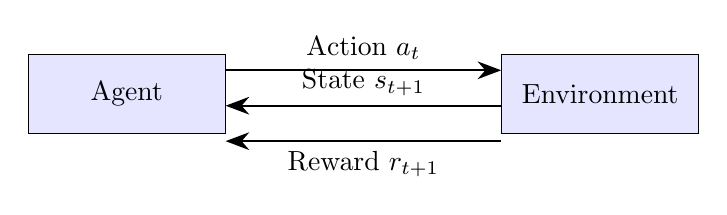
\begin{tikzpicture}[
    node distance=2.5cm,
    block/.style={rectangle, draw, minimum width=2.5cm, minimum height=1cm, align=center, fill=blue!10},
    arrow/.style={-{Stealth[length=3mm]}, thick}
]
    % Agent
    \node[block] (agent) {Agent};

    % Environment
    \node[block, right=3.5cm of agent] (env) {Environment};

    % Arrows
    \draw[arrow] ([yshift=0.3cm]agent.east) -- node[above] {Action $a_t$} ([yshift=0.3cm]env.west);
    \draw[arrow] ([yshift=-0.15cm]env.west) -- node[above] {State $s_{t+1}$} ([yshift=-0.15cm]agent.east);
    \draw[arrow] ([yshift=-0.6cm]env.west) -- node[below] {Reward $r_{t+1}$} ([yshift=-0.6cm]agent.east);

\end{tikzpicture}
\caption{The agent-environment interaction in a Markov Decision Process. At each time step, the agent observes state $s_t$, takes action $a_t$, and receives reward $r_{t+1}$ along with the next state $s_{t+1}$.}
\label{fig:mdp}
\end{figure}

\subsection{Value Functions and Bellman Equations}

Value functions are central to reinforcement learning, as they estimate how good it is for an agent to be in a given state or to take a given action. The \textbf{state-value function} $V^\pi(s)$ gives the expected return when starting in state $s$ and following policy $\pi$ thereafter:
\begin{equation}
V^\pi(s) = \mathbb{E}_\pi[G_t | s_t = s] = \mathbb{E}_\pi\left[\sum_{k=0}^{\infty} \gamma^k R_{t+k+1} \middle| s_t = s\right]
\end{equation}

The \textbf{action-value function} (or Q-function) $Q^\pi(s,a)$ gives the expected return when starting in state $s$, taking action $a$, and following policy $\pi$ thereafter:
\begin{equation}
Q^\pi(s,a) = \mathbb{E}_\pi[G_t | s_t = s, a_t = a]
\end{equation}

These value functions satisfy recursive relationships known as the \textbf{Bellman equations}, which express the value of a state in terms of the values of successor states. For the state-value function:
\begin{equation}
V^\pi(s) = \sum_{a \in \mathcal{A}} \pi(a|s) \sum_{s' \in \mathcal{S}} P(s'|s,a)[R(s,a) + \gamma V^\pi(s')]
\end{equation}

The optimal value functions are defined as the maximum value achievable over all policies:
\begin{align}
V^*(s) &= \max_\pi V^\pi(s) \\
Q^*(s,a) &= \max_\pi Q^\pi(s,a)
\end{align}

The optimal value functions satisfy the \textbf{Bellman optimality equations}:
\begin{equation}
Q^*(s,a) = \sum_{s' \in \mathcal{S}} P(s'|s,a)\left[R(s,a) + \gamma \max_{a' \in \mathcal{A}} Q^*(s',a')\right]
\end{equation}

Once we have the optimal Q-function $Q^*$, we can extract the optimal policy through $\pi^*(s) = \arg\max_{a \in \mathcal{A}} Q^*(s,a)$. This greedy policy with respect to $Q^*$ is guaranteed to be optimal.

\subsection{Value-Based Methods}

Value-based methods learn the optimal value function and derive a policy from it. The foundational algorithm in this category is Q-learning \cite{watkins1992q}, which updates Q-values using:
\begin{equation}
Q(s_t, a_t) \leftarrow Q(s_t, a_t) + \alpha \left[R_{t+1} + \gamma \max_{a} Q(s_{t+1}, a) - Q(s_t, a_t)\right]
\end{equation}
where $\alpha$ is the learning rate. The term in brackets is the temporal difference (TD) error, measuring the discrepancy between the current estimate and the bootstrapped target.

For problems with large or continuous state spaces, tabular methods become infeasible. Deep Q-Networks (DQN) address this limitation by using deep neural networks as function approximators for the Q-function \cite{mnih2015human}. DQN introduces two critical innovations that stabilize training. \textbf{Experience replay} stores transitions $(s_t, a_t, r_{t+1}, s_{t+1})$ in a replay buffer and samples mini-batches uniformly for training, breaking temporal correlations and improving sample efficiency. The \textbf{target network} maintains a separate copy of the Q-network with parameters $\theta^-$ that are periodically synchronized with the main network, preventing the instability that arises from chasing a constantly moving target.

The DQN loss function is:
\begin{equation}
L(\theta) = \mathbb{E}_{(s,a,r,s') \sim \mathcal{D}}\left[\left(r + \gamma \max_{a'} Q(s',a';\theta^-) - Q(s,a;\theta)\right)^2\right]
\end{equation}

Several improvements to the basic DQN algorithm have been proposed. \textbf{Double DQN} \cite{van2016deep} addresses the overestimation bias by decoupling action selection from action evaluation, using the online network to select actions and the target network to evaluate them. \textbf{Dueling DQN} \cite{wang2016dueling} separates the Q-function into value and advantage streams: $Q(s,a) = V(s) + A(s,a) - \frac{1}{|\mathcal{A}|}\sum_{a'} A(s,a')$, enabling the network to learn state values independently of action advantages. \textbf{Prioritized Experience Replay} \cite{schaul2016prioritized} samples transitions based on their TD error magnitude, focusing learning on the most informative experiences. \textbf{Noisy Networks} \cite{fortunato2018noisy} replace deterministic layers with noisy ones, providing state-dependent exploration without requiring epsilon-greedy schedules.

\begin{figure}[H]
\centering
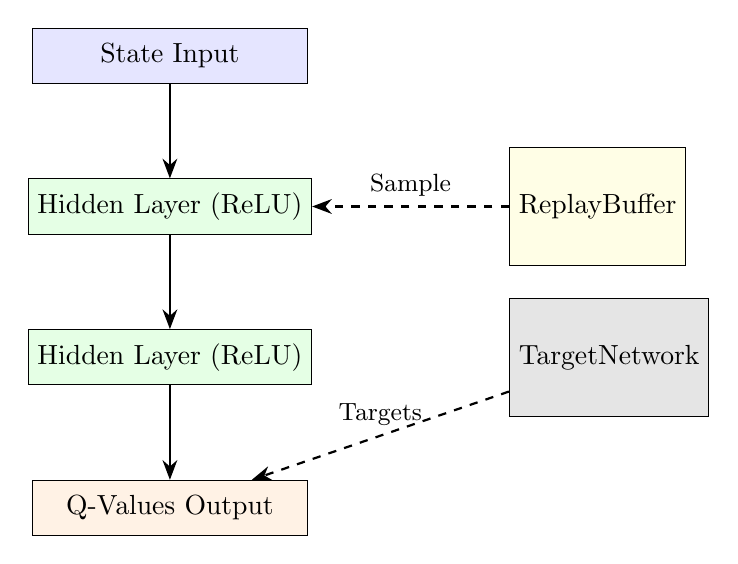
\begin{tikzpicture}[
    node distance=1.2cm,
    layer/.style={rectangle, draw, minimum width=3.5cm, minimum height=0.7cm, align=center},
    arrow/.style={-{Stealth[length=2.5mm]}, thick}
]
    % Main network
    \node[layer, fill=blue!10] (input) {State Input};
    \node[layer, fill=green!10, below=of input] (hidden1) {Hidden Layer (ReLU)};
    \node[layer, fill=green!10, below=of hidden1] (hidden2) {Hidden Layer (ReLU)};
    \node[layer, fill=orange!10, below=of hidden2] (output) {Q-Values Output};

    \draw[arrow] (input) -- (hidden1);
    \draw[arrow] (hidden1) -- (hidden2);
    \draw[arrow] (hidden2) -- (output);

    % Replay buffer
    \node[rectangle, draw, fill=yellow!10, minimum width=2cm, minimum height=1.5cm, right=2.5cm of hidden1] (buffer) {Replay\\Buffer};

    % Target network
    \node[rectangle, draw, fill=gray!20, minimum width=2cm, minimum height=1.5cm, right=2.5cm of hidden2] (target) {Target\\Network};

    % Connections
    \draw[arrow, dashed] (buffer) -- node[above, font=\small] {Sample} (hidden1);
    \draw[arrow, dashed] (target) -- node[above, font=\small] {Targets} (output);

\end{tikzpicture}
\caption{DQN architecture showing the main Q-network, experience replay buffer, and target network. The replay buffer stores transitions and provides decorrelated training samples, while the target network provides stable learning targets.}
\label{fig:dqn}
\end{figure}

\subsection{Policy Gradient Methods}

While value-based methods learn a value function and derive a policy from it, policy gradient methods directly parameterize and optimize the policy $\pi_\theta(a|s)$. The objective is to maximize the expected return:
\begin{equation}
J(\theta) = \mathbb{E}_{\tau \sim \pi_\theta}[G(\tau)]
\end{equation}

The policy gradient theorem \cite{williams1992simple} provides a way to compute gradients of this objective:
\begin{equation}
\nabla_\theta J(\theta) = \mathbb{E}_{\tau \sim \pi_\theta}\left[\sum_{t=0}^T \nabla_\theta \log \pi_\theta(a_t|s_t) G_t\right]
\end{equation}

The \textbf{REINFORCE} algorithm uses Monte Carlo estimation of this gradient, updating parameters after each complete episode. To reduce variance, a baseline $b(s_t)$ is subtracted from the return, with the state-value function $V(s_t)$ being a common choice. This leads to the advantage function $A(s,a) = Q(s,a) - V(s)$, which measures how much better an action is compared to the average.

\textbf{Actor-Critic} methods combine value-based and policy-based approaches. The actor (policy network) selects actions while the critic (value network) evaluates them, providing lower-variance gradient estimates. The \textbf{Advantage Actor-Critic (A2C)} algorithm uses the TD error as an estimate of the advantage:
\begin{equation}
A(s_t, a_t) \approx r_{t+1} + \gamma V(s_{t+1}) - V(s_t)
\end{equation}

\textbf{Proximal Policy Optimization (PPO)} \cite{schulman2017proximal} has become one of the most popular RL algorithms due to its simplicity and effectiveness. Building on Trust Region Policy Optimization (TRPO) \cite{schulman2015trust}, PPO constrains policy updates to prevent large, destabilizing changes using a clipped surrogate objective:
\begin{equation}
L^{CLIP}(\theta) = \mathbb{E}_t\left[\min\left(r_t(\theta)A_t, \text{clip}(r_t(\theta), 1-\epsilon, 1+\epsilon)A_t\right)\right]
\end{equation}
where $r_t(\theta) = \frac{\pi_\theta(a_t|s_t)}{\pi_{\theta_{old}}(a_t|s_t)}$ is the probability ratio. The clipping prevents the policy from changing too drastically in a single update. PPO also uses Generalized Advantage Estimation (GAE) \cite{schulman2016high} to balance bias and variance in advantage estimates:
\begin{equation}
A_t^{GAE} = \sum_{l=0}^{\infty} (\gamma\lambda)^l \delta_{t+l}
\end{equation}
where $\delta_t = r_t + \gamma V(s_{t+1}) - V(s_t)$ is the TD error and $\lambda$ controls the trade-off.

\begin{figure}[H]
\centering
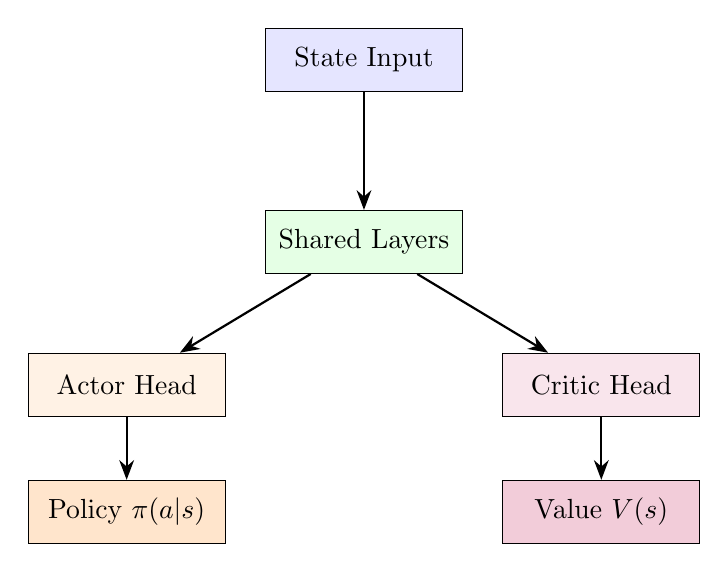
\begin{tikzpicture}[
    node distance=1.5cm,
    block/.style={rectangle, draw, minimum width=2.5cm, minimum height=0.8cm, align=center},
    arrow/.style={-{Stealth[length=2.5mm]}, thick}
]
    % Input
    \node[block, fill=blue!10] (input) {State Input};

    % Shared layers
    \node[block, fill=green!10, below=of input] (shared) {Shared Layers};

    % Actor branch
    \node[block, fill=orange!10, below left=1cm and 0.5cm of shared] (actor) {Actor Head};
    \node[block, fill=orange!20, below=0.8cm of actor] (policy) {Policy $\pi(a|s)$};

    % Critic branch
    \node[block, fill=purple!10, below right=1cm and 0.5cm of shared] (critic) {Critic Head};
    \node[block, fill=purple!20, below=0.8cm of critic] (value) {Value $V(s)$};

    % Arrows
    \draw[arrow] (input) -- (shared);
    \draw[arrow] (shared) -- (actor);
    \draw[arrow] (shared) -- (critic);
    \draw[arrow] (actor) -- (policy);
    \draw[arrow] (critic) -- (value);

\end{tikzpicture}
\caption{Actor-Critic architecture used in PPO and A2C. The actor outputs action probabilities while the critic estimates state values. Both can share lower layers for feature extraction.}
\label{fig:actor_critic}
\end{figure}

\subsection{Multi-Agent Reinforcement Learning}

Multi-agent RL extends single-agent RL to scenarios with multiple decision-makers, modeled as stochastic games \cite{lowe2017multi}. In our two-snake competitive setting, each agent $i$ has its own policy $\pi^i$ and receives individual rewards $R^i$. The key challenge is non-stationarity: from each agent's perspective, the environment appears non-stationary because other agents' policies change during training.

Several approaches address multi-agent training. \textbf{Independent Q-Learning} treats other agents as part of the environment, with each agent learning independently using standard DQN. While simple, this approach may not converge to Nash equilibria. \textbf{Self-play} trains a single agent against copies of itself, creating a natural curriculum as the opponent improves. \textbf{Curriculum learning} progressively increases opponent difficulty, starting from static opponents and advancing through random, scripted, and finally learning opponents.

For competitive snake, we employ a five-stage curriculum. In Stage 0, the agent faces a static opponent that does not move, allowing it to learn basic food collection. Stage 1 introduces a random opponent that takes uniformly random actions. Stage 2 uses a greedy opponent that always moves toward the nearest food. Stage 3 freezes a trained policy as the opponent, preventing information leakage during training. Finally, Stage 4 enables co-evolution where both agents learn simultaneously.

%==============================================================================
% SECTION 3: EXPERIMENTS
%==============================================================================
\section{Experiments}

This section describes our experimental setup for training reinforcement learning agents to play Snake. We detail the environment implementations, state representations, network architectures, and training procedures for both single-snake and competitive two-snake scenarios.

\subsection{Environment Design}

We implemented Snake game environments following the Gymnasium API standard, ensuring compatibility with modern reinforcement learning frameworks. The single-snake environment features a configurable grid (default $10 \times 10$) where the snake starts with length 3 at the center. Food appears randomly on empty cells, and episodes terminate upon collision with walls or the snake's body, or after a timeout.

The action space uses relative directions: STRAIGHT (0), RIGHT\_TURN (1), and LEFT\_TURN (2). This relative action space reduces learning complexity as the agent only needs to decide how to adjust its trajectory rather than selecting from absolute directions. The timeout mechanism terminates episodes if the snake fails to collect food within $grid\_size^2 \times 2$ steps, preventing infinite wandering while allowing arbitrarily long episodes when progress is made.

For competitive scenarios, we implemented a two-snake environment where both snakes share the grid and compete for food. A round ends when one snake reaches a target food count or when a snake dies. Victory rewards are substantial (+100) to encourage winning behavior, while death penalties (-50 to -100) discourage reckless play. The two-snake environment supports both classic (CPU-based) and vectorized (GPU-accelerated) implementations.

We developed GPU-accelerated vectorized environments using PyTorch tensors, enabling parallel training of 128-256 simultaneous games. This vectorization achieves 100-300x speedup compared to sequential training, making extensive hyperparameter searches and longer training runs feasible. The vectorized environments maintain identical game logic while batching all operations for GPU efficiency.

\subsection{State Representations}

State representation significantly impacts learning efficiency and final performance. We designed multiple representations with increasing sophistication, ranging from basic 11-dimensional feature vectors to comprehensive 24-dimensional representations.

The simplest representation uses 11 dimensions capturing immediate spatial awareness. This includes three binary danger indicators for collision risk in relative directions (straight, right, left), four binary food direction indicators showing whether food lies up, right, down, or left relative to the head, and four one-hot encoded features representing the snake's current absolute direction. This basic representation provides sufficient information for learning fundamental navigation skills.

Building on this foundation, we developed a 14-dimensional representation that adds flood-fill features. These three additional features measure the ratio of reachable cells in each relative direction using breadth-first search. By computing how much free space is accessible from potential next positions, the agent can avoid moves leading to dead-ends or self-trapping situations. The flood-fill computation normalizes values by the maximum possible free cells, producing features in the range [0, 1].

Further extensions include a 19-dimensional selective representation that adds tail-related features (direction to tail and normalized distance), helping the snake follow its tail for safety in dense configurations. The most comprehensive 24-dimensional enhanced representation adds escape route counts, tail reachability via flood-fill, and snake length ratio. While providing rich information, this representation incurs higher computational cost that may not justify the marginal performance improvement.

For CNN-based approaches, we use a grid representation with 3 channels encoding head position, body position, and food position respectively. This raw grid input requires convolutional layers to extract spatial features but provides complete spatial information without hand-crafted feature engineering.

For competitive two-snake scenarios, we designed a 35-dimensional competitive representation. This combines self-awareness features (danger, food direction, current direction, flood-fill), opponent-awareness features (opponent body danger, head position relative to self, opponent direction, opponent length, distance to opponent, threat level), and competitive metrics (length difference, food count difference, food proximity advantage, space control ratio).

\begin{figure}[H]
\centering
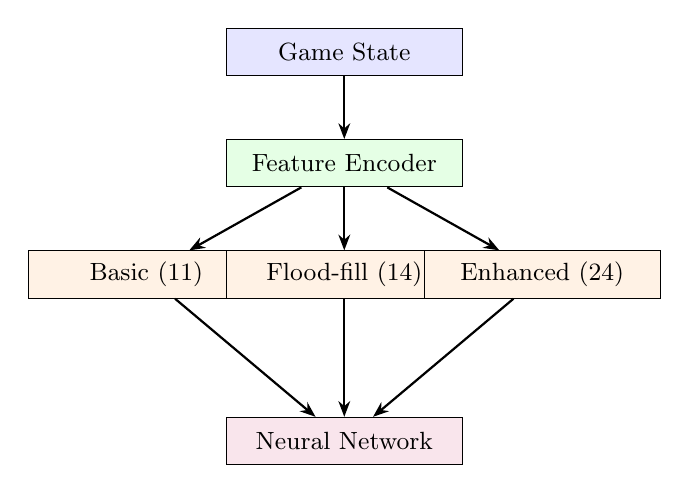
\begin{tikzpicture}[
    node distance=0.8cm,
    box/.style={rectangle, draw, minimum width=3cm, minimum height=0.6cm, align=center, font=\small},
    arrow/.style={-{Stealth[length=2mm]}, thick}
]
    % State input
    \node[box, fill=blue!10] (state) {Game State};

    % Encoder
    \node[box, fill=green!10, below=of state] (encoder) {Feature Encoder};

    % Features
    \node[box, fill=orange!10, below left=0.8cm and -0.5cm of encoder] (basic) {Basic (11)};
    \node[box, fill=orange!10, below=of encoder] (flood) {Flood-fill (14)};
    \node[box, fill=orange!10, below right=0.8cm and -0.5cm of encoder] (enhanced) {Enhanced (24)};

    % Network
    \node[box, fill=purple!10, below=1.5cm of flood] (network) {Neural Network};

    \draw[arrow] (state) -- (encoder);
    \draw[arrow] (encoder) -- (basic);
    \draw[arrow] (encoder) -- (flood);
    \draw[arrow] (encoder) -- (enhanced);
    \draw[arrow] (basic) -- (network);
    \draw[arrow] (flood) -- (network);
    \draw[arrow] (enhanced) -- (network);

\end{tikzpicture}
\caption{State representation pipeline showing different feature extraction options. The flood-fill representation provides the best balance between information content and computational cost.}
\label{fig:state_rep}
\end{figure}

\subsection{Reward Shaping}

The reward function guides learning behavior. For single-snake, we use food consumption (+10), collision/death (-10), and time penalty (-0.01 per step). The time penalty provides dense feedback encouraging efficient food collection rather than aimless wandering. Some experiments include distance-based shaping ($\pm 1$ for moving toward/away from food) to accelerate early learning.

For competitive two-snake, rewards are more complex. Food consumption gives +10, death results in -50 to -100 depending on configuration, winning the round yields +100, and the opponent dying while the agent survives provides +50. The step penalty is reduced or removed to focus on strategic play rather than speed.

\subsection{Network Architectures}

For MLP-based agents (feature input), we use two hidden layers with 128 neurons each and ReLU activations. Larger networks (256x256) are used for competitive scenarios requiring more capacity. The output layer produces Q-values (for DQN) or action logits (for policy gradient methods).

For CNN-based agents (grid input), we use three convolutional layers (32, 64, 64 filters with 3x3 kernels), followed by a fully connected layer (256 neurons) and the output layer. Padding preserves spatial dimensions through the convolutional layers.

PPO uses separate actor and critic networks, or a shared backbone with separate heads. The actor outputs action logits processed through softmax for action probabilities. The critic outputs a single scalar value estimate.

\subsection{Baseline Algorithms}

To contextualize RL agent performance, we implemented several deterministic baseline algorithms. The random baseline selects actions uniformly at random, providing a lower bound on expected performance. The greedy food baseline uses A* pathfinding to navigate toward the nearest food, representing a simple but effective heuristic. The shortest path baseline employs Dijkstra's algorithm considering both walls and the snake's body as obstacles, representing near-optimal navigation when sufficient free space exists. These baselines establish performance benchmarks against which learning algorithms can be compared.

\subsection{Training Procedures}

We implemented training scripts for all algorithms with consistent interfaces and configurable hyperparameters. Table \ref{tab:hyperparameters} summarizes key hyperparameters.

\begin{table}[H]
\centering
\caption{Training Hyperparameters}
\label{tab:hyperparameters}
\begin{tabular}{lcc}
\toprule
\textbf{Parameter} & \textbf{DQN} & \textbf{PPO} \\
\midrule
Learning rate & 0.001 & 0.0003 \\
Discount factor ($\gamma$) & 0.99 & 0.99 \\
Batch size & 64 & 64 \\
Buffer/Rollout size & 100,000 & 2,048 \\
Hidden layers & 128x128 & 128x128 \\
$\epsilon$ start/end & 1.0/0.01 & N/A \\
$\epsilon$ decay & 0.995 & N/A \\
Clip parameter & N/A & 0.2 \\
GAE $\lambda$ & N/A & 0.95 \\
Entropy coefficient & N/A & 0.01 \\
Target update freq & 1,000 steps & N/A \\
\bottomrule
\end{tabular}
\end{table}

For DQN variants, we train for 5,000-10,000 episodes with 256 parallel environments. Training uses Adam optimizer with gradient clipping (max norm 1.0). The replay buffer stores transitions and samples uniformly (or by priority for PER). The target network updates every 1,000 training steps.

For policy gradient methods, we collect rollouts of 2,048 steps across parallel environments, then perform multiple epochs (4-10) of mini-batch updates. PPO uses the clipped objective with value function and entropy bonuses. A2C uses simpler advantage estimation without clipping.

For two-snake curriculum training, we progress through five stages with increasing opponent difficulty. Each stage trains until a win rate threshold is achieved (70\% for static, 60\% for random, 55\% for greedy, 50\% for frozen) or a maximum step count is reached. The final co-evolution stage trains both agents simultaneously.

\subsection{Single-Snake Results}

We trained all algorithms and recorded learning curves. Figures \ref{fig:dqn_results} through \ref{fig:reinforce_results} show training progress for each algorithm.

\begin{figure}[H]
\centering
\includegraphics[width=0.9\textwidth]{../results/figures/dqn_training_20251125_172020.png}
\caption{DQN training curves showing episode rewards, scores, and moving averages over training.}
\label{fig:dqn_results}
\end{figure}

\begin{figure}[H]
\centering
\includegraphics[width=0.9\textwidth]{../results/figures/ppo_training_20251125_172040.png}
\caption{PPO training curves demonstrating faster convergence and higher final performance compared to DQN.}
\label{fig:ppo_results}
\end{figure}

\begin{figure}[H]
\centering
\includegraphics[width=0.9\textwidth]{../results/figures/double_dqn_training_20251125_172121.png}
\caption{Double DQN training showing reduced overestimation compared to vanilla DQN.}
\label{fig:double_dqn}
\end{figure}

\begin{figure}[H]
\centering
\includegraphics[width=0.9\textwidth]{../results/figures/dueling_dqn_training_20251125_172132.png}
\caption{Dueling DQN training demonstrating improved learning through value-advantage separation.}
\label{fig:dueling_dqn}
\end{figure}

\begin{figure}[H]
\centering
\includegraphics[width=0.9\textwidth]{../results/figures/a2c_training_20251125_172050.png}
\caption{A2C training curves showing on-policy learning dynamics.}
\label{fig:a2c_results}
\end{figure}

\begin{figure}[H]
\centering
\includegraphics[width=0.9\textwidth]{../results/figures/reinforce_training_20251125_172102.png}
\caption{REINFORCE training demonstrating high variance typical of Monte Carlo policy gradients.}
\label{fig:reinforce_results}
\end{figure}

\subsection{Two-Snake Competitive Results}

Competitive training proved more challenging, requiring curriculum learning for stable performance. Figure \ref{fig:two_snake_classic} shows classic DQN two-snake training, while Figure \ref{fig:curriculum} shows curriculum learning progression.

\begin{figure}[H]
\centering
\includegraphics[width=0.9\textwidth]{../results/figures/two_snake_classic_training_20251125_172440.png}
\caption{Classic two-snake DQN training showing competitive dynamics between agents.}
\label{fig:two_snake_classic}
\end{figure}

\begin{figure}[H]
\centering
\includegraphics[width=0.9\textwidth]{../results/figures/ppo_two_snake_curriculum_20251125_172509.png}
\caption{PPO curriculum learning showing progressive improvement across five training stages.}
\label{fig:curriculum}
\end{figure}

\begin{figure}[H]
\centering
\includegraphics[width=0.9\textwidth]{../results/figures/dqn_two_snake_curriculum_20251125_172523.png}
\caption{DQN curriculum learning demonstrating stage-by-stage progression against increasingly difficult opponents.}
\label{fig:dqn_curriculum}
\end{figure}

%==============================================================================
% SECTION 4: DISCUSSION
%==============================================================================
\section{Discussion}

This section analyzes experimental results, discusses key findings, and examines challenges encountered during development.

\subsection{Performance Analysis}

Our experiments reveal several important patterns in algorithm performance. PPO with flood-fill features consistently achieves the highest scores in single-snake scenarios, demonstrating the effectiveness of policy gradient methods for this task. The flood-fill representation proves critical for avoiding self-trapping, a common failure mode where the snake blocks its own escape routes.

DQN variants show varying degrees of improvement over vanilla DQN. Double DQN reduces overestimation and provides more stable learning. Dueling DQN shows benefits when many actions have similar values, which occurs frequently in open grid positions. Prioritized Experience Replay accelerates learning by focusing on high-error transitions but requires careful tuning of priority parameters. Noisy networks eliminate the need for epsilon scheduling but require sufficient training to learn appropriate exploration levels.

CNN-based approaches consistently underperform MLP-based approaches with feature engineering. This counterintuitive result suggests that hand-crafted features capturing spatial relationships (particularly flood-fill) provide more relevant information than raw grid inputs for this relatively small-scale problem. CNNs may show advantages for larger grids or more complex visual environments.

For two-snake competitive scenarios, curriculum learning proves essential. Direct co-evolution often fails to produce capable agents, as both snakes learn to avoid each other rather than compete effectively. The staged curriculum allows agents to first master basic skills before facing adaptive opponents.

\subsection{Key Findings}

The flood-fill feature emerges as the most impactful state representation enhancement. By measuring reachable free space, it enables the agent to avoid moves that lead to dead-ends, a critical capability as the snake grows longer. Without this feature, even well-trained agents frequently trap themselves.

Policy gradient methods (especially PPO) outperform value-based methods for Snake. We attribute this to PPO's stable updates and entropy regularization, which maintain exploration throughout training. DQN's epsilon-greedy exploration becomes less effective as epsilon decays, potentially causing the agent to exploit suboptimal policies.

The vectorized GPU environments provide 100-300x speedup, transforming training from hours to minutes for typical configurations. This parallelization approach shares conceptual similarities with Asynchronous Advantage Actor-Critic (A3C) \cite{mnih2016asynchronous}, which uses parallel workers for diverse experience collection. Our synchronous vectorized approach achieves similar benefits while being simpler to implement on GPU hardware.

In competitive scenarios, asymmetric agent sizes (larger network for the main agent) combined with curriculum learning produce the best results. The curriculum stages each contribute differently: static opponents teach basic movement, random opponents teach robustness, greedy opponents teach competition, and frozen opponents prevent co-adaptation artifacts.

\subsection{Challenges Encountered}

Exploration-exploitation balance posed significant challenges. Too much exploration (high epsilon) prevents learning, while too little causes premature convergence to suboptimal policies. We found exponential epsilon decay (0.995 per episode) effective for DQN, while PPO's entropy bonus provides more stable exploration.

Sparse rewards in Snake (only receiving signal upon eating food or dying) slow early learning. Distance-based reward shaping accelerates initial progress but must be carefully scaled to avoid distorting the optimal policy. We found small shaping rewards ($\pm 1$) effective without causing problematic shortcuts.

Two-snake credit assignment is difficult because outcomes depend on both agents' actions. When one snake dies, determining whether this resulted from its own mistake or the opponent's skill is ambiguous. Curriculum learning helps by initially removing this ambiguity (against deterministic opponents).

Computational efficiency required significant optimization. Initial implementations suffered from excessive training frequency (training too often relative to data collection) and sequential operations that could be batched. Profiling and optimization yielded a 2.5x speedup in overall training time.

%==============================================================================
% SECTION 5: LIMITATIONS AND FUTURE OF RL
%==============================================================================
\section{Limitations and Future of Reinforcement Learning}

\subsection{Current Limitations}

Despite achieving reasonable performance, our approach has several limitations. Sample efficiency remains a concern: training requires millions of environment steps to achieve competent play. While vectorization helps, more sample-efficient algorithms (model-based RL, offline RL) could reduce data requirements.

Hyperparameter sensitivity affects reproducibility. Different random seeds produce varying results, and hyperparameters optimized for one grid size may not transfer to others. Automated hyperparameter search could address this but increases computational costs.

Generalization is limited. Agents trained on 10x10 grids perform poorly on 20x20 grids without retraining. The state representation (particularly feature dimensions) is fixed, preventing direct transfer. Approaches like domain randomization or meta-learning could improve generalization.

The maximum achievable score depends on snake length becoming unmanageable. As the snake grows, maintaining survival becomes increasingly difficult. Our agents typically plateau at scores significantly below the theoretical maximum (grid size squared minus initial length).

\subsection{Future Directions}

Several promising directions could extend this work. Rainbow DQN \cite{hessel2018rainbow} combines all DQN improvements (Double, Dueling, PER, Noisy, N-step, Distributional) into a single algorithm. Implementing Rainbow for Snake would provide a strong value-based baseline.

Hierarchical RL could decompose the problem into high-level planning (path to food) and low-level control (collision avoidance). This structure matches the natural hierarchy in Snake strategy and could improve both learning efficiency and interpretability.

Transfer learning between grid sizes would increase practical applicability. Techniques like progressive networks or policy distillation could enable knowledge transfer from smaller to larger grids.

For competitive scenarios, population-based training could evolve diverse strategies rather than converging to a single equilibrium. This would produce more robust agents capable of handling varied opponent behaviors.

\subsection{Broader Reinforcement Learning Landscape}

Reinforcement learning continues advancing rapidly. Large-scale RL has achieved remarkable results, from AlphaFold's protein structure prediction to ChatGPT's RL from Human Feedback (RLHF) for language model alignment. These applications demonstrate RL's versatility beyond game playing.

Offline RL trains agents on fixed datasets without environment interaction, enabling RL in domains where online exploration is costly or dangerous. Decision Transformer recasts RL as sequence modeling, leveraging transformer architectures that have revolutionized natural language processing.

Multi-agent RL is increasingly important for applications like autonomous driving, where multiple vehicles must coordinate. Techniques for handling non-stationarity, emergent communication, and cooperation continue developing.

Safety and robustness remain critical challenges as RL systems are deployed in real-world applications. Ensuring agents behave safely under distributional shift, adversarial inputs, and specification gaming requires ongoing research.

%==============================================================================
% SECTION 6: CONCLUSION
%==============================================================================
\section{Conclusion}

This project comprehensively investigated reinforcement learning techniques applied to the Snake game. We implemented multiple algorithms spanning value-based methods (DQN with Double, Dueling, PER, and Noisy variants) and policy gradient methods (REINFORCE, A2C, PPO), evaluated them in both single-snake and competitive two-snake scenarios, and identified key factors affecting performance.

Our main contributions include implementing GPU-accelerated vectorized environments achieving 100-300x speedup, designing and comparing multiple state representations with flood-fill features proving most impactful, demonstrating that PPO with flood-fill features achieves superior single-snake performance, developing effective curriculum learning strategies for competitive two-snake training, and providing practical recommendations for algorithm and representation selection.

Key takeaways for practitioners include using flood-fill features to prevent self-trapping behaviors, preferring PPO for stable training with good final performance, employing curriculum learning for competitive or multi-agent scenarios, and leveraging GPU vectorization for efficient experimentation.

This work demonstrates that classic games remain valuable testbeds for RL research, providing accessible environments for algorithm development while presenting genuine challenges in state representation, reward design, and training stability. The techniques and insights developed here extend to more complex sequential decision-making problems in robotics, game AI, and autonomous systems.

%==============================================================================
% REFERENCES
%==============================================================================
\bibliographystyle{IEEEtran}
\begin{thebibliography}{99}

\bibitem{sutton2018reinforcement}
R.~S. Sutton and A.~G. Barto, \emph{Reinforcement Learning: An Introduction}, 2nd ed. MIT Press, 2018.

\bibitem{mnih2015human}
V.~Mnih \emph{et al.}, ``Human-level control through deep reinforcement learning,'' \emph{Nature}, vol. 518, no. 7540, pp. 529--533, 2015.

\bibitem{silver2016mastering}
D.~Silver \emph{et al.}, ``Mastering the game of Go with deep neural networks and tree search,'' \emph{Nature}, vol. 529, no. 7587, pp. 484--489, 2016.

\bibitem{watkins1992q}
C.~J. Watkins and P.~Dayan, ``Q-learning,'' \emph{Machine Learning}, vol. 8, no. 3-4, pp. 279--292, 1992.

\bibitem{van2016deep}
H.~van Hasselt, A.~Guez, and D.~Silver, ``Deep reinforcement learning with Double Q-learning,'' in \emph{Proc. AAAI Conf. Artificial Intelligence}, 2016.

\bibitem{wang2016dueling}
Z.~Wang \emph{et al.}, ``Dueling network architectures for deep reinforcement learning,'' in \emph{Proc. Int. Conf. Machine Learning}, 2016.

\bibitem{schaul2016prioritized}
T.~Schaul, J.~Quan, I.~Antonoglou, and D.~Silver, ``Prioritized experience replay,'' in \emph{Proc. Int. Conf. Learning Representations}, 2016.

\bibitem{fortunato2018noisy}
M.~Fortunato \emph{et al.}, ``Noisy networks for exploration,'' in \emph{Proc. Int. Conf. Learning Representations}, 2018.

\bibitem{williams1992simple}
R.~J. Williams, ``Simple statistical gradient-following algorithms for connectionist reinforcement learning,'' \emph{Machine Learning}, vol. 8, no. 3-4, pp. 229--256, 1992.

\bibitem{schulman2017proximal}
J.~Schulman, F.~Wolski, P.~Dhariwal, A.~Radford, and O.~Klimov, ``Proximal policy optimization algorithms,'' \emph{arXiv preprint arXiv:1707.06347}, 2017.

\bibitem{schulman2016high}
J.~Schulman, P.~Moritz, S.~Levine, M.~Jordan, and P.~Abbeel, ``High-dimensional continuous control using generalized advantage estimation,'' in \emph{Proc. Int. Conf. Learning Representations}, 2016.

\bibitem{lowe2017multi}
R.~Lowe \emph{et al.}, ``Multi-agent actor-critic for mixed cooperative-competitive environments,'' in \emph{Proc. Neural Information Processing Systems}, 2017.

\bibitem{mnih2016asynchronous}
V.~Mnih \emph{et al.}, ``Asynchronous methods for deep reinforcement learning,'' in \emph{Proc. Int. Conf. Machine Learning}, 2016.

\bibitem{hessel2018rainbow}
M.~Hessel \emph{et al.}, ``Rainbow: Combining improvements in deep reinforcement learning,'' in \emph{Proc. AAAI Conf. Artificial Intelligence}, 2018.

\bibitem{schulman2015trust}
J.~Schulman, S.~Levine, P.~Abbeel, M.~Jordan, and P.~Moritz, ``Trust region policy optimization,'' in \emph{Proc. Int. Conf. Machine Learning}, 2015.

\end{thebibliography}

\end{document}
